%%%%%%%%%%%%%%%%%%%%%%%%%%%%%%%%%%%%%%%%%%%%%%%%%%%%%%%%%%%%%%%%%%%%%%%%%%%%%%%%
%2345678901234567890123456789012345678901234567890123456789012345678901234567890
%        1         2         3         4         5         6         7         8

\documentclass[letterpaper, 12 pt, conference]{ieeeconf}  % Comment this line out
                                                          % if you need a4paper
%\documentclass[a4paper, 10pt, conference]{ieeeconf}      % Use this line for a4
                                                          % paper

\IEEEoverridecommandlockouts                              % This command is only
                                                          % needed if you want to
                                                          % use the \thanks command
\overrideIEEEmargins
% See the \addtolength command later in the file to balance the column lengths
% on the last page of the document



% The following packages can be found on http:\\www.ctan.org
%\usepackage{graphics} % for pdf, bitmapped graphics files
%\usepackage{epsfig} % for postscript graphics files
%\usepackage{mathptmx} % assumes new font selection scheme installed
%\usepackage{times} % assumes new font selection scheme installed
\usepackage{amsmath} % assumes amsmath package installed
\usepackage{amssymb}  % assumes amsmath package installed
\usepackage{bm}
\usepackage{graphicx}
\usepackage{color}
\usepackage{subfig}
\usepackage{url}
\usepackage{xcolor}
\usepackage{pdfpages}
\usepackage{float}
%\usepackage{enumitem}
\usepackage{algorithmicx}
\usepackage{algpseudocode}
\usepackage{multicol}

 \title{\LARGE \bf Visual Filtering of Large Energy Consumption Datasets by Leveraging Usage Clusters
 }

 \author{
 Diego Arguelles%
  \thanks{MBA student, Graduate School of Business, Stanford University, {\tt\small dargu10@stanford.edu}.}
    \and 
    Ramon Iglesias%
  \thanks{Graduate student, Department of Civil and Environmental Engineering, Stanford University, {\tt\small rdit@stanford.edu}.}
 }

\begin{document}

\maketitle

\begin{abstract}
In this paper, we present a method of visually exploring large energy consumption datasets. By leveraging previous work on clustering smart meter patterns, the resulting visualization enables users to efficiently explore a large spatio-temporal dataset. This work takes place in the larger context of VISDOM, a web application that enables energy stakeholders to host and explore large smart meter datasets.
\end{abstract}

\section{Introduction}

% data is exploding

% stress in the power grid

% efforts to manipulate behavior

% lack of specialized methods for existing stakeholders

% VISDOM is addressing this spot

% The issue of capturing patterns in large datasets

For about a hundred years, the electricity and utility model in the United States remained virtually unchanged: large-scale, centralized generation built, owned and operated by utility companies which, using large distribution networks, delivered power to thousands of households. Over the past decade, this model has been challenged and taken to its limits.


The growth of distributed energy generation coupled with the explosion of residential and commercial solar systems (enabled by lower costs of PV cells and innovative financial structures) has dramatically changed the existing utility model in the US. This has created great challenges and opportunities for a diverse set of stakeholders -from startups to large-scale utility companies.


Several of these stakeholder groups have begun harnessing the power of Big Data to understand market dynamics and identifying opportunities and threats to the system. For example, California PG\&E began installing smart meters into their clients’ households. This in turn allowed the company to go from 1 reading per month, to 12 per minute.


As a response to this, a group of scientists at Stanford University - June Flora, Chin-Woo Tan, Sam Borgeson, and Professor Ram Rajagopal- built an open-source platform to begin harnessing the power of this new information: the Visualization and Insight System for Demand Operations and Management (VISDOM). The next step for the team is to begin developing innovative tools to help stakeholders generate insightful and actionable analysis. 
VISDOM has data for ~100K households from PG\&E’s consumer base. The tool holds information on zip codes, dates, daily consumption and several readings within each day. More importantly, the VISDOM team can generate the specific consumption pattern for any 24 hour period for any household in the sample. Furthermore, the VISDOM team has successfully typified consumption patterns into ~200 dictionary types. 


This project set out to develop an innovative way to filteringer this massive data set into spatial-temporal clusters. It aims to inform decisions ranging from rate structures to incentive programs as well as identify target markets for businesses and other commercial endeavors. 

\section{Motivation}

The problem is interesting due to it’s importance and practical relevance. The changes we’ve seen over the past decade have fundamentally challenged a system design that’s been the foundation of the world for the past century. 


The problem is difficult due to several issues:


First, the amount of data is massive: there are 12 million households in California alone! Each of them has a unique consumption pattern that is not static but, rather, changes daily.


Second, there is a large amount of variables, some of which are easy to filter with (e.g. average daily consumption, date, etc.). Yet, the truly crucial variable –consumption pattern- is difficult to interact with since 1) it can take a large number of values (currently +200 dictionary types exist), 2) it is nominal in nature and 3) it is best explained graphically.


Providing users a way to efficiently interact with this variable is key to developing interesting clusters that can result in actionable decisions


Finally, there’s a challenge in drawing actionable impact from this large amount of data. We have decided to focus on generating spatial-temporal clusters to inform decision makers –from utilities planning demand to legislators approving rate structures. These method will allow an insightful interaction with data that educates decisions.


\section{Related Work}

% Spatio temporal Viz

% Latency in interactive visualizations

% Energy pattern Clustering

% Web Application viz

The problem of visualizing spatio-temporal datasets has been an ongoing research avenue for several centuries, e.g. \cite{minard1869tableaux}, but its relevance has been heightened with the proliferation of large datasets and the democratization of geographical applications. Traditional approaches to cartographic visualizations, such as choropleths and heatmaps, in the browser have been increasingly available since the birth of Google Maps in 2005, allowing users to build custom static displays of geographical information. Additionally, the need to find insights a,cross multiple dimensions has led the push for technological innovations in the creation of interactive maps \cite{leaflet,mapbox,2011-d3}. 


However, the unprecedented data explosion poses a challenge when creating effective interactive visualizations. On one hand, it is necessary to portray visualizations that genuinely represent the truth, on the other, the massive size of the datasets imply that subsequent queries become computationally expensive, and from the user’s perspective, time consuming. Indeed, \cite{liu2014effects}, shows that a delay a small as 500ms may incur significant costs to user experience and the data set coverage. Thus, it is paramount for visualization experts to devise methods to query and display interactive visualizations in time spans that are within the human attention capacity. Such effort can be seen in \cite{lins2013nanocubes}, where they propose a data structure that fit in browser memory to store precomputed queries, resulting in fast interactive visualizations of millions of data points. Other methods include sampling the original dataset, as in \cite{park2015visualization} where a method to draw random samples is proposed such that the resulting visualization retains the same visual characteristics.

Perhaps the most traditional method to draw insights from data is to use statistics. However, when doing so in the context of interactive graphics, it is important to reach levels of abstraction in which the user can perform its own questions. In \cite{kwac2014household}, the authors propose a clustering method for energy usage that later gets leveraged in the VISDOM web application \cite{borgeson2015learning}. Our work in this project builds on top of these papers to provide fast and high fidelity visualizations that can be included in the VISDOM platform.

\section{Approach}

It was essential to work close to the VISDOM team to understand the opportunities and needs of this tool. Several interviews were conducted, resulting in identifying a need around filtering via the “dictionary types”. “Dictionary types” are a set of ~200 archetypical consumption patterns into which (using statistical analysis) each household’s patterns are categorized into. Despite having a code, the best way to interact with these types is via their graphical representation.


On the other hand, in order to generate truly actionable insights (for a diverse set of stakeholders), there was a need to generate results in the form of clusters. Given the types of decisions, said clusters required several dimensions, most importantly, geographical and temporal.


Thus, our approach was to generate an interactive visualization with all the relevant filters that, simultaneously delivers actionable clusters. The key, innovative element here was visual filtering on the dictionary types. This was done via a d3 implementation of the brush methods –as suggested by Hochheiser and Shneiderman in their “Visual Queries for Finding Patterns in Time Series Data” paper. Although the original application of this method was around querying for time series, we believe applying it to consumption patterns would bring a new sense of clarity to the VISDOM application. We included additional more “familiar” filters built around this idea of visual filtering.



\section{Methods}

% Daily Consumption Clustering

% Time Search on Clusters

% D3 Update Pattern

% D3 Brushes and Crossfilters


Three aspects of the dataset were of particular interest to the VISDOM team: daily consumption patterns, yearly seasonal behavior, and spatial distribution. Thus, our visualization was divided in these three views. Additionally, since our visualization is meant to be used via a browser, three web technologies were key for the implementation: D3 \cite{2011-d3}, Crossfilter \cite{crossfilter}, and Leaflet \cite{leaflet}.

\paragraph{Daily Consumption View} The key insight of this paper is that it is computationally more efficient and cognitively more informative to query daily consumption patterns in the "dictionary type" space. Thus, the Daily Consumption View (DCV) displays to the user all 200 dictionary type profiles, with the $x$-axis defining the time of consumption and the $y$-axis the fraction of the daily consumption. Moreover, the interaction of this view is similar to the traditional Time Search \cite{hochheiser2001interactive} visualication, where the user can dynamically create multiple brushes to select dictionaries with specific characteristics. 

To avoid overloading the user with unnecessary information, the dictionary profiles are grayed out to signalize that they are have not been selected. This also serves the purpose of guiding the user of where to look. However, since browser computation time tends to increase significantly with the number of SVG elements, we implemented the unselected dictionaries with a HTML Canvas overlay. Thus, the number of SVG elements would be reduced to only those being selected, naturally a much smaller subset. In order to speed up queries in this view, we leveraged D3's quadtree search functionality. This allowed us to keep the query time within 30ms, regardless of the brush area. 

\paragraph{Yearly Consumption View} While the DCV allows the user to explore patterns on a daily basis, the Yearly Consumption View (YCV) allows the user to see patterns throughout the year. The visualization consists of a bar chart with dates in the $x$-axis and total daily consumption in the $y$-axis. Since the visualization changes with each DCV query, the scale of the $y$-axis is dynamically adjusted to reflect the domain of the resulting data. This allows users to keep a grasp of the magnitude of energy being consumed without losing the ability to detect variations within the chart. Like the DCV, the YCV is equipped with a brush in the time dimension, allowing users to query a specific period of time

\paragraph{Zipcode Choropleth} In contrast to the other two views, the Zipcode Choropleth (ZC) displays the total energy used in the time span selected in the YCV that fits the patterns selected in the DCV. Thus, the ZC satisfies the necessity to connect spatial component to the two time aspects. Since the number of zip code areas in California is large (~2,500), efficiently handling updates to the polygons became a major concern. Two methods were primarily used to reduce the rerender time. First, leveraging the D3 update pattern made it possible to reduce the number of polygon updates in each query. However, D3 does not handle well when the updates are on existing data. Thus, two sets of polygon data are stored in memory to "trick" to trigger the D3 update functions correctly. Second, by encoding the polygons as a TopoJSON instead of a GeoJSON we were able to reduce the size of the geographical dataset (TopoJSON uses only one path instead of two for polygon boundaries).

\paragraph{Crossfiltering} Finally, to glue the three views, we used the Crossfilter \cite{crossfilter} module. This made the propagation of queries across different views relatively easy.

\section{Results}

\begin{figure*}[tb]
\centering
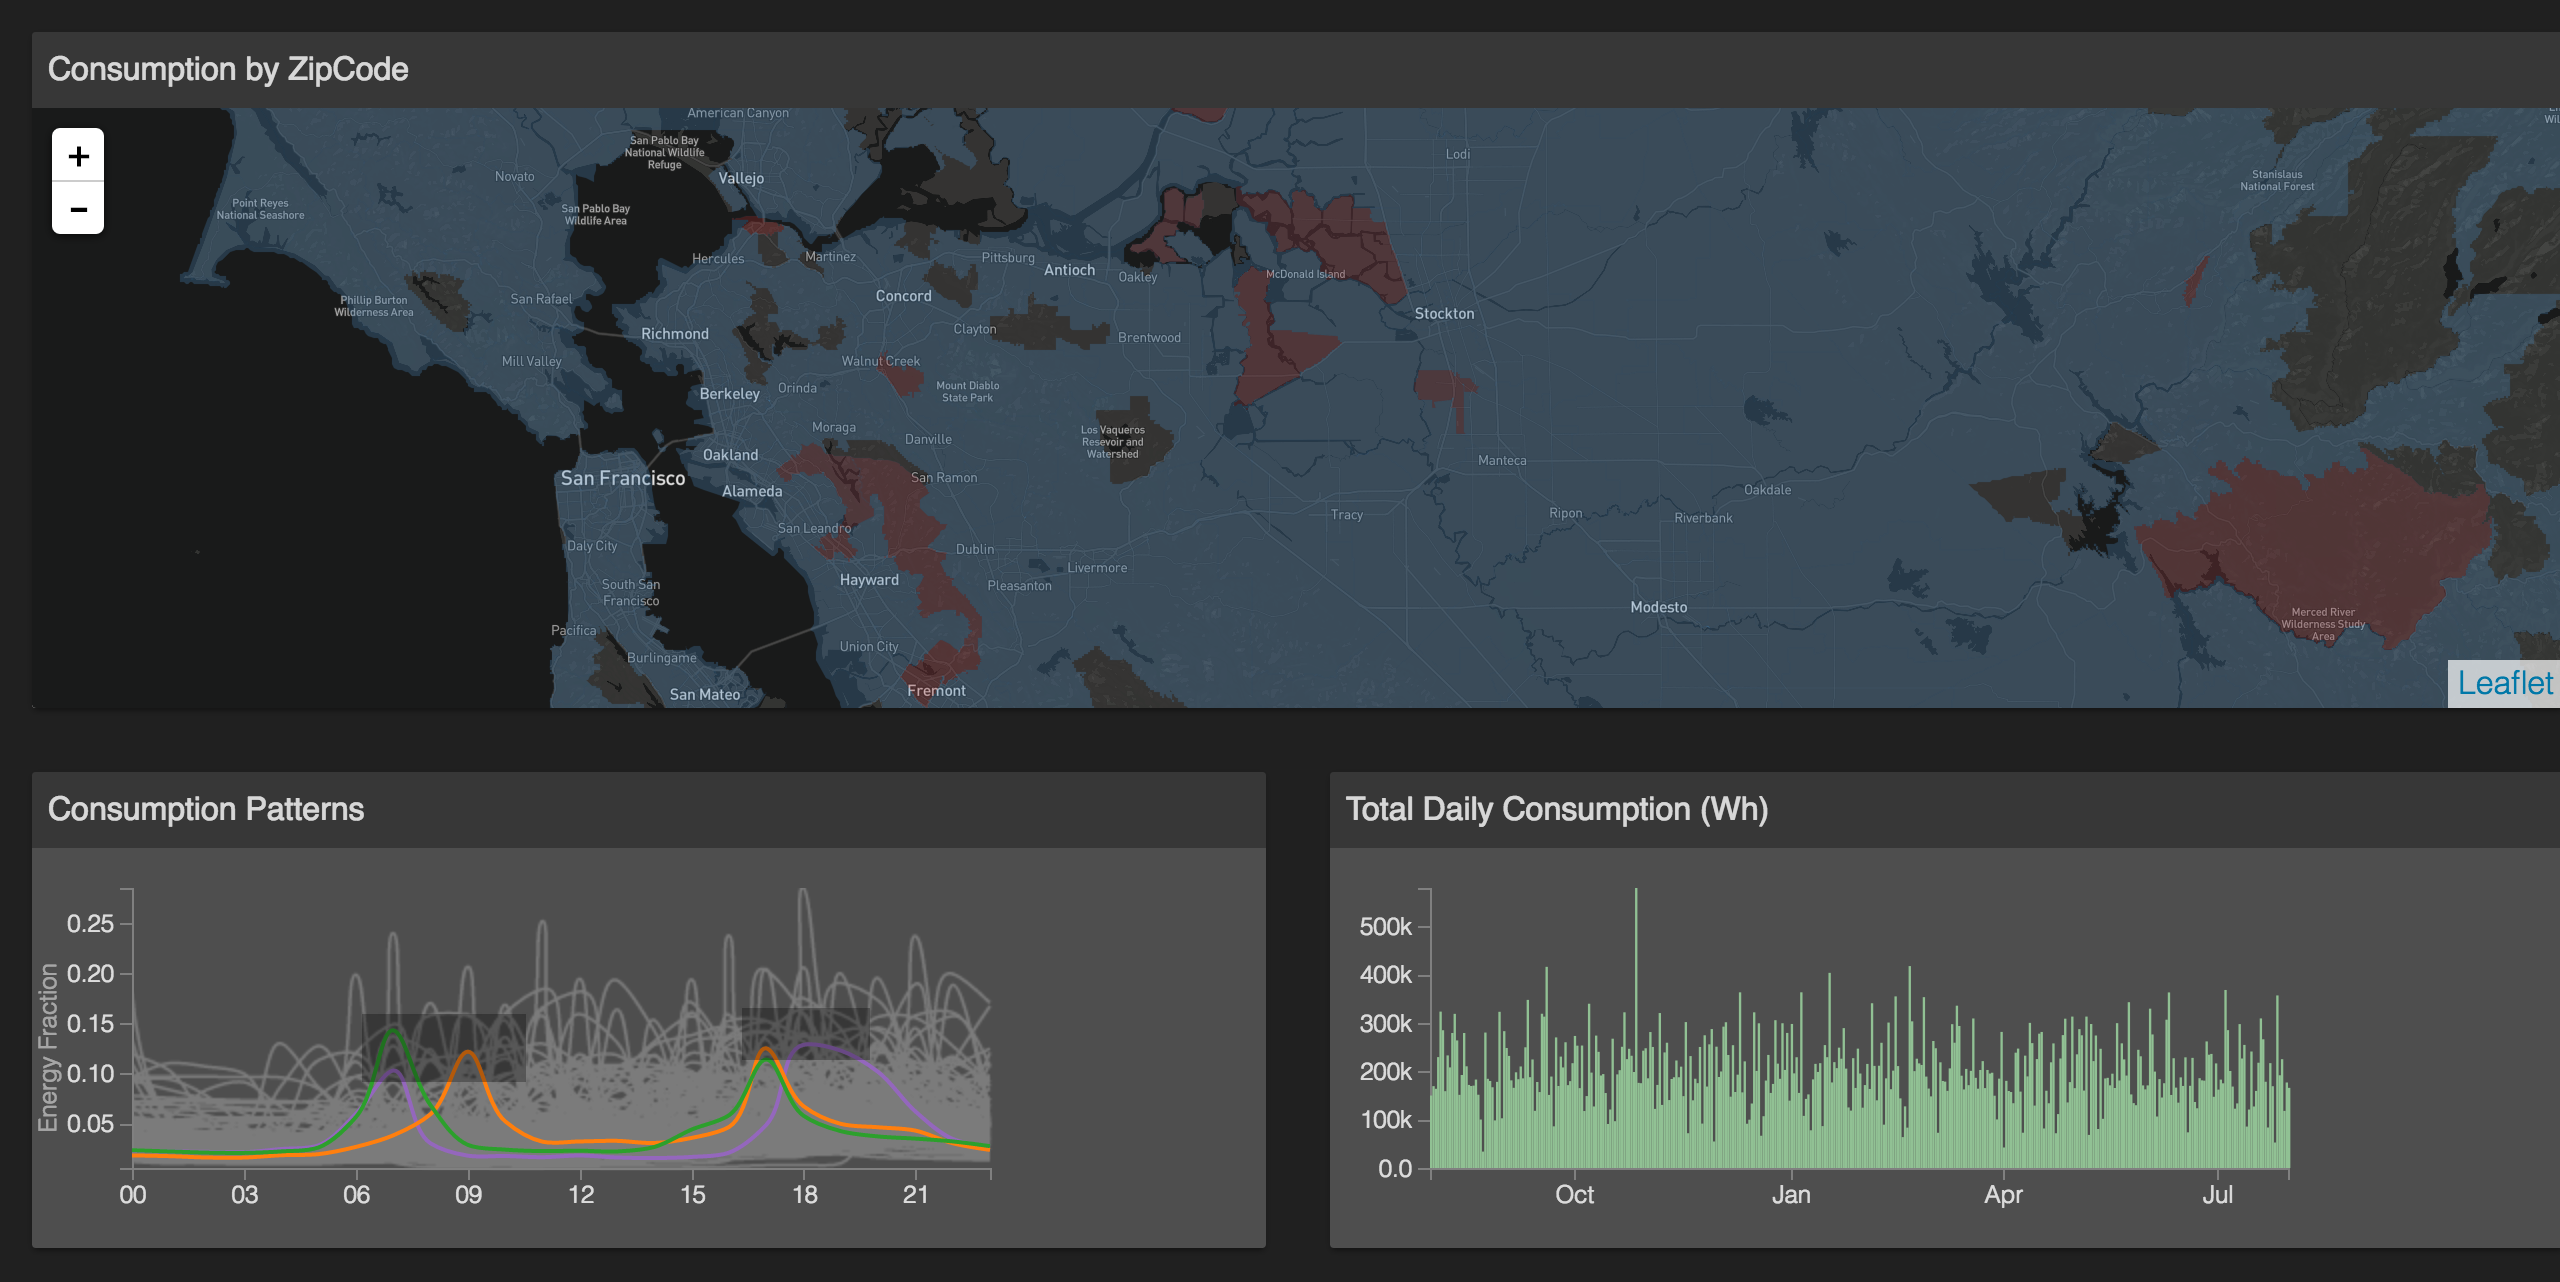
\includegraphics[width=\textwidth]{screenshot.png}
\caption{caption}
\label{fig:viz}
\end{figure*}


% Web application

% Time Responsiveness

% Spatial and Time components

% using the YCV as a movie

% Tests

% rerender time

The resulting visualization can be seen in Figure \ref{fig:viz}, with the ZC on top, the DCV on the bottom left and the YCV on the bottom right. We tested its operation with a set of 2,000 customers with a year long consumption history. Overall, the visualization is quite efficient, most re-render operations are within 100ms, queries on the DCV are within 50ms, and even faster for the YCV. This makes the utilization of the visualization feasible. 

The reception from the VISDOM team has so far been quite successful. The usage of dictionary types for visual filtering strengthens the value of their research. While we have yet to find interesting patterns that span the three views, some of the members like the idea of using the YCV as a "play movie" mechanism, by creating a small brush and moving it around the year. Finally, the technologies in which the visualization is built makes it easy to attach it to the VISDOM application, which is an aspect appreciated by the developers of VISDOM.

\section{Future Work and Conclusion}

The implementation was successful in providing users with a tool to filter on the key variable in the data set. This allows users to explore the data in a more intuitive, seamless manner by interacting with the key variable in the most appropriate way possible. Applying visual querying is often an efficient and effective way to filter large amounts of data. The applications of this method are sure to increase in the future.

The results of this project have been promising and  encourage further exploration in the intersection between visualization and the VISDOM team. Specifically, there are three areas of future work that would be interesting to explore in the near future.


First, the mechanics of this implementation are exceptional at aggregating data. Yet, the flip side of this is a likely loss of precision. An interesting area of study would be to understand the optimal level of aggregation that maximizes user’s ease of interaction while still delivering output at a level appropriate for decision making, What precise, targeted output can be developed beyond current tools.


Second, an energy expert who interacted with the tool mentioned an interest in developing an interphase in which the user “drew” the desired queries. In other words, would it be possible to substitute the current box/ brush implementation for an interactive pen/ tablet interface. Nonetheless, this solution would still likely result in user-generated inaccuracy -see the point above.


Finally, and most importantly, to take this tool further, extensive user interviews are required. It would be important to test the tools not only with the VISDOM team but include a diverse set of potential end-users. As mentioned at the beginning of this paper, the energy industry is undergoing massive changes and now has a more diverse set of stakeholders than in previous decades. It would be important to test the implementation with some or all of the following groups: utility companies, academic researchers, solar and other distributive generation companies, micro-grid and storage firms, policy makers and start-ups. Gaining a view into their interaction as well as remaining needs would help guide the next steps of this tool.


% This works very well

% Will integrate to VISDOM

% Larger Datasets

% Sampling methods

% Other potential filters

% Arbitrary pattern matching

The implementation was successful in providing users with a tool to filter on the key variable in the data set. This allows users to explore the data in a more intuitive, seamless manner by interacting with the key variable in the most appropriate way possible.


Applying visual querying is often an efficient and effective way to filter large amounts of data. The applications of this method are sure to increase in the future.


\bibliographystyle{unsrt} 
\bibliography{ref.bib}

\end{document}